\subsection{SMODERP2D entering an open source world}\label{ref:open_source_providers}

SMODERP2D is the project with a long history. Over the years its
development has been driven by the Department of Landscape Water
Conservation at the Czech Technical University in Prague. In 2018
SMODERP2D developers started working on a new generation of the model
in order to solve or at least to improve various critical issues of
the project (see SMODERP2D logo in Figure~\ref{fig:smoderp2d_logo}). 
This includes most importantly the computation stability
and performance, better interoperability, and lack of
documentation. Recently SMODERP2D source code has been published on
GitHub \cite{smoderp2d-github-2019} under GNU GPL licence in order to
attract a wider audience, new developers and users.

\begin{figure}[ht!]
  {\tiny
\begin{verbatim}

       @ @ @   @       @     @ @     @ @ @     @ @ @ @  @ @ @    @ @ @
      @        @ @   @ @   @     @   @     @   @        @     @  @     @
      @        @   @   @  @       @  @      @  @        @     @  @     @
        @ @    @       @  @       @  @      @  @ @ @    @ @ @    @ @ @
            @  @       @  @       @  @      @  @        @   @    @
            @  @       @   @     @   @     @   @        @    @   @
       @ @ @   @       @     @ @     @ @ @     @ @ @ @  @     @  @

      \  \  /   / /    \   \  /   \  /    /     /        @ @ @   @ @ @
       \ _\/   /_/      \   \/     \/    /_____/        @     @  @     @
           \__/          \  /      _\___/                     @  @      @
               \____      \/      /                          @   @      @
                    \_____/______/                         @     @      @
                                 \                       @       @     @
                                  \____________________ @ @ @ @  @ @ @
\end{verbatim}
}
\caption{ASCII-art SMODERP2D project logo}
\label{fig:smoderp2d_logo}
\end{figure}

The model is implemented in Python programming language using the
object-oriented paradigm. The original source code has been designed
with a low level of scalability, limited readability and
interoperability. Part of the computation phase responsible for a data
preparation was restricted to a single platform only, Esri ArcGIS. In
2018 the original source code has been completely refactorized. Python
classes defining computational steps were re-organized in a
hierarchical manner. Major design-related changes have been done in
Python classes responsible for data handling and preparation using GIS
software tools. Data preparation workflow is handled by a
newly-defined a base, partly abstract Python class ({\tt BaseProvider}
in Figure~\ref{fig:uml_diagram}). Functionality depending on used
GIS package has been separated into new classes. This step was crucial
in order to make data preparation workflow GIS package
independent. The only supported platform, Esri ArcGIS, has been
separated from a base workflow. Based on that, a new concept of
so-called {\em GIS providers} has been introduced, see
Figure \ref{fig:uml_diagram}. 

\begin{figure}[ht!]
  \begin{center}
    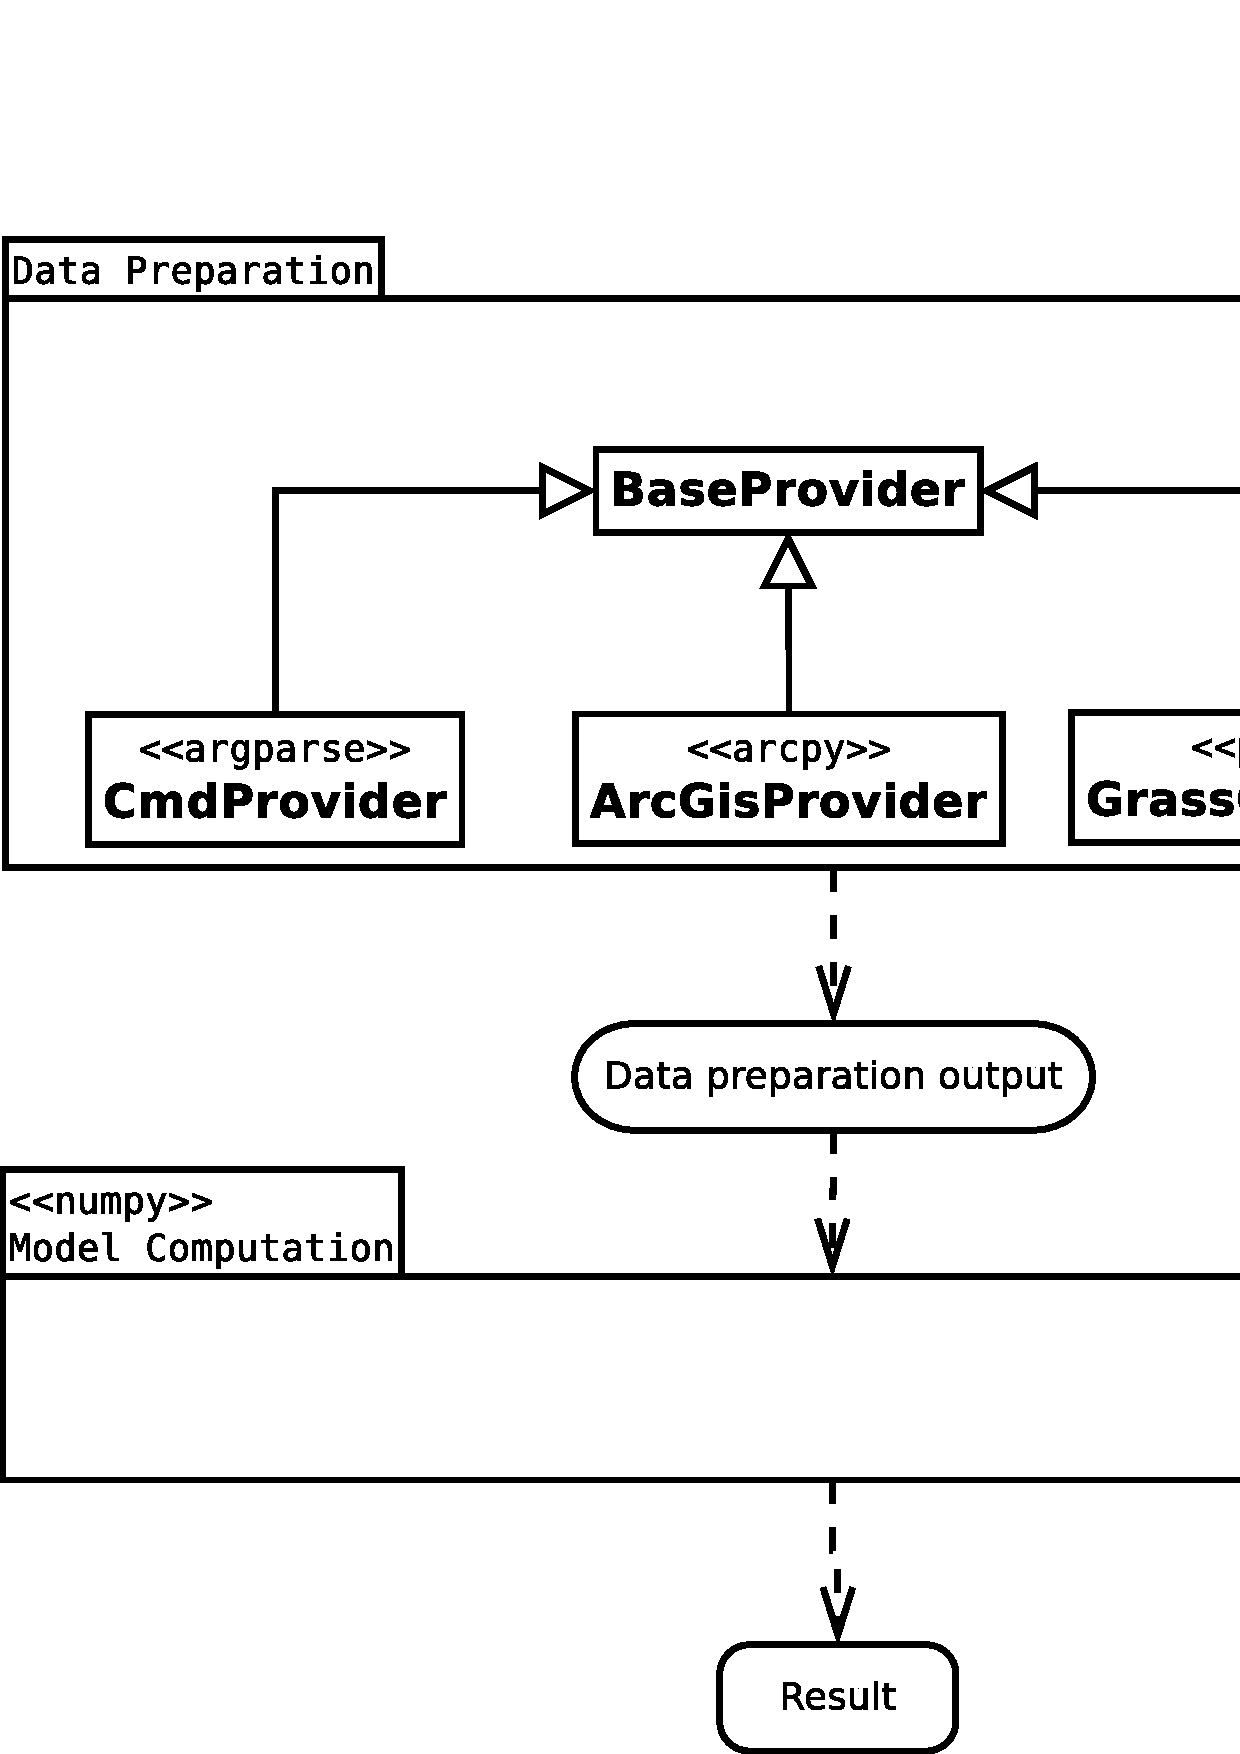
\includegraphics[width=0.8\columnwidth]{figures/uml_diagram.pdf}
    \caption{Concept of GIS providers (software dependecies outlined by stereotypes)}
    \label{fig:uml_diagram}
  \end{center}
\end{figure}

The key point is the separation of GIS functionality related code from
the~generic workflow defined by the base provider. The base provider
depends only on standard builtin Python libraries. Array-like
computation is performed by a well-known NumPy library. Using GIS
provider prototypes, the SMODERP2D project can be easily extended to
support other GIS packages. Currently, the SMODERP2D project comes
with three different GIS providers. Support for Esri ArcGIS platform
is implemented by {\tt ArcGISProvider}, GRASS GIS is handled by {\tt
  GrassGisProvider}, see \ref{sec:grass_provider}. The {\tt
  CmdProvider} is triggered only when the model computation is run
from a command-line. In this case, it is assumed that the data
preparation phase has been already performed by one of supported GIS
platforms.

Example of running computation from a command-line bellow. Option {\it
  --typecomp roff} specifies that only model computation without data
preparation phase is triggered. It means that data has been already
preprocessed and stored in a pickle file distributed by a {\it test.ini}
configuration file.

\begin{verbatim}
python ./bin/start-smoderp2d.py --typecomp roff \
 --indata tests/test.ini
\end{verbatim}

\subsubsection{GRASS GIS integration}\label{sec:grass_provider}
SMODERP2D supported GIS platforms have been recerently extended by a
+new GRASS-based GIS provider. Introducing an open source GIS platform
to SMODERP2D workflow is crucial from the perspective of
interoperability. SMODERP2D users can choose between a proprietary
Esri ArcGIS platform and an open source GRASS GIS
\cite{neteler2012grass}. The GRASS GIS provider is designed similarly
to ArcGIS provider. From a Python perspective, there is only one
difference, GIS functions are accessed by PyGRASS package
\cite{ijgi2010201}. Nevertheless, an integration of GRASS tools in the
SMODERP2D project required a few improvements in GRASS GIS
itself. That was possible since GRASS GIS is an open source project
distributed under GNU GPL licence. These improvements have been
integrated into main distribution and will be part of upcoming GRASS
GIS version 7.8. A GRASS {\em v.to.points} module
\cite{v-to-points-2019} has been extended to extract from lines start
or end nodes only. This functionality is used to determine the slope
of a polyline stream feature to ensure that its direction will always
be downslope. Another
improvement is related to a {\em v.to.db} GRASS module
\cite{v-to-db-2019}. This tool allows uploading geometry-related
information into the attribute table. 
%% JJ: co co jsem do nasledujici vety dopsal nevim jestl je uplne pravda
Newly added option {\it
next\_edge} allows adding information about the next left and right
edge based on the segment orientation determined from surface slope. 
This functionality is important for SMODERP2D in order to
determine stream network correct connectivity as
Figure~\ref{fig:stream_next_edge} shows.

\begin{figure}[ht!]
  \begin{center}
    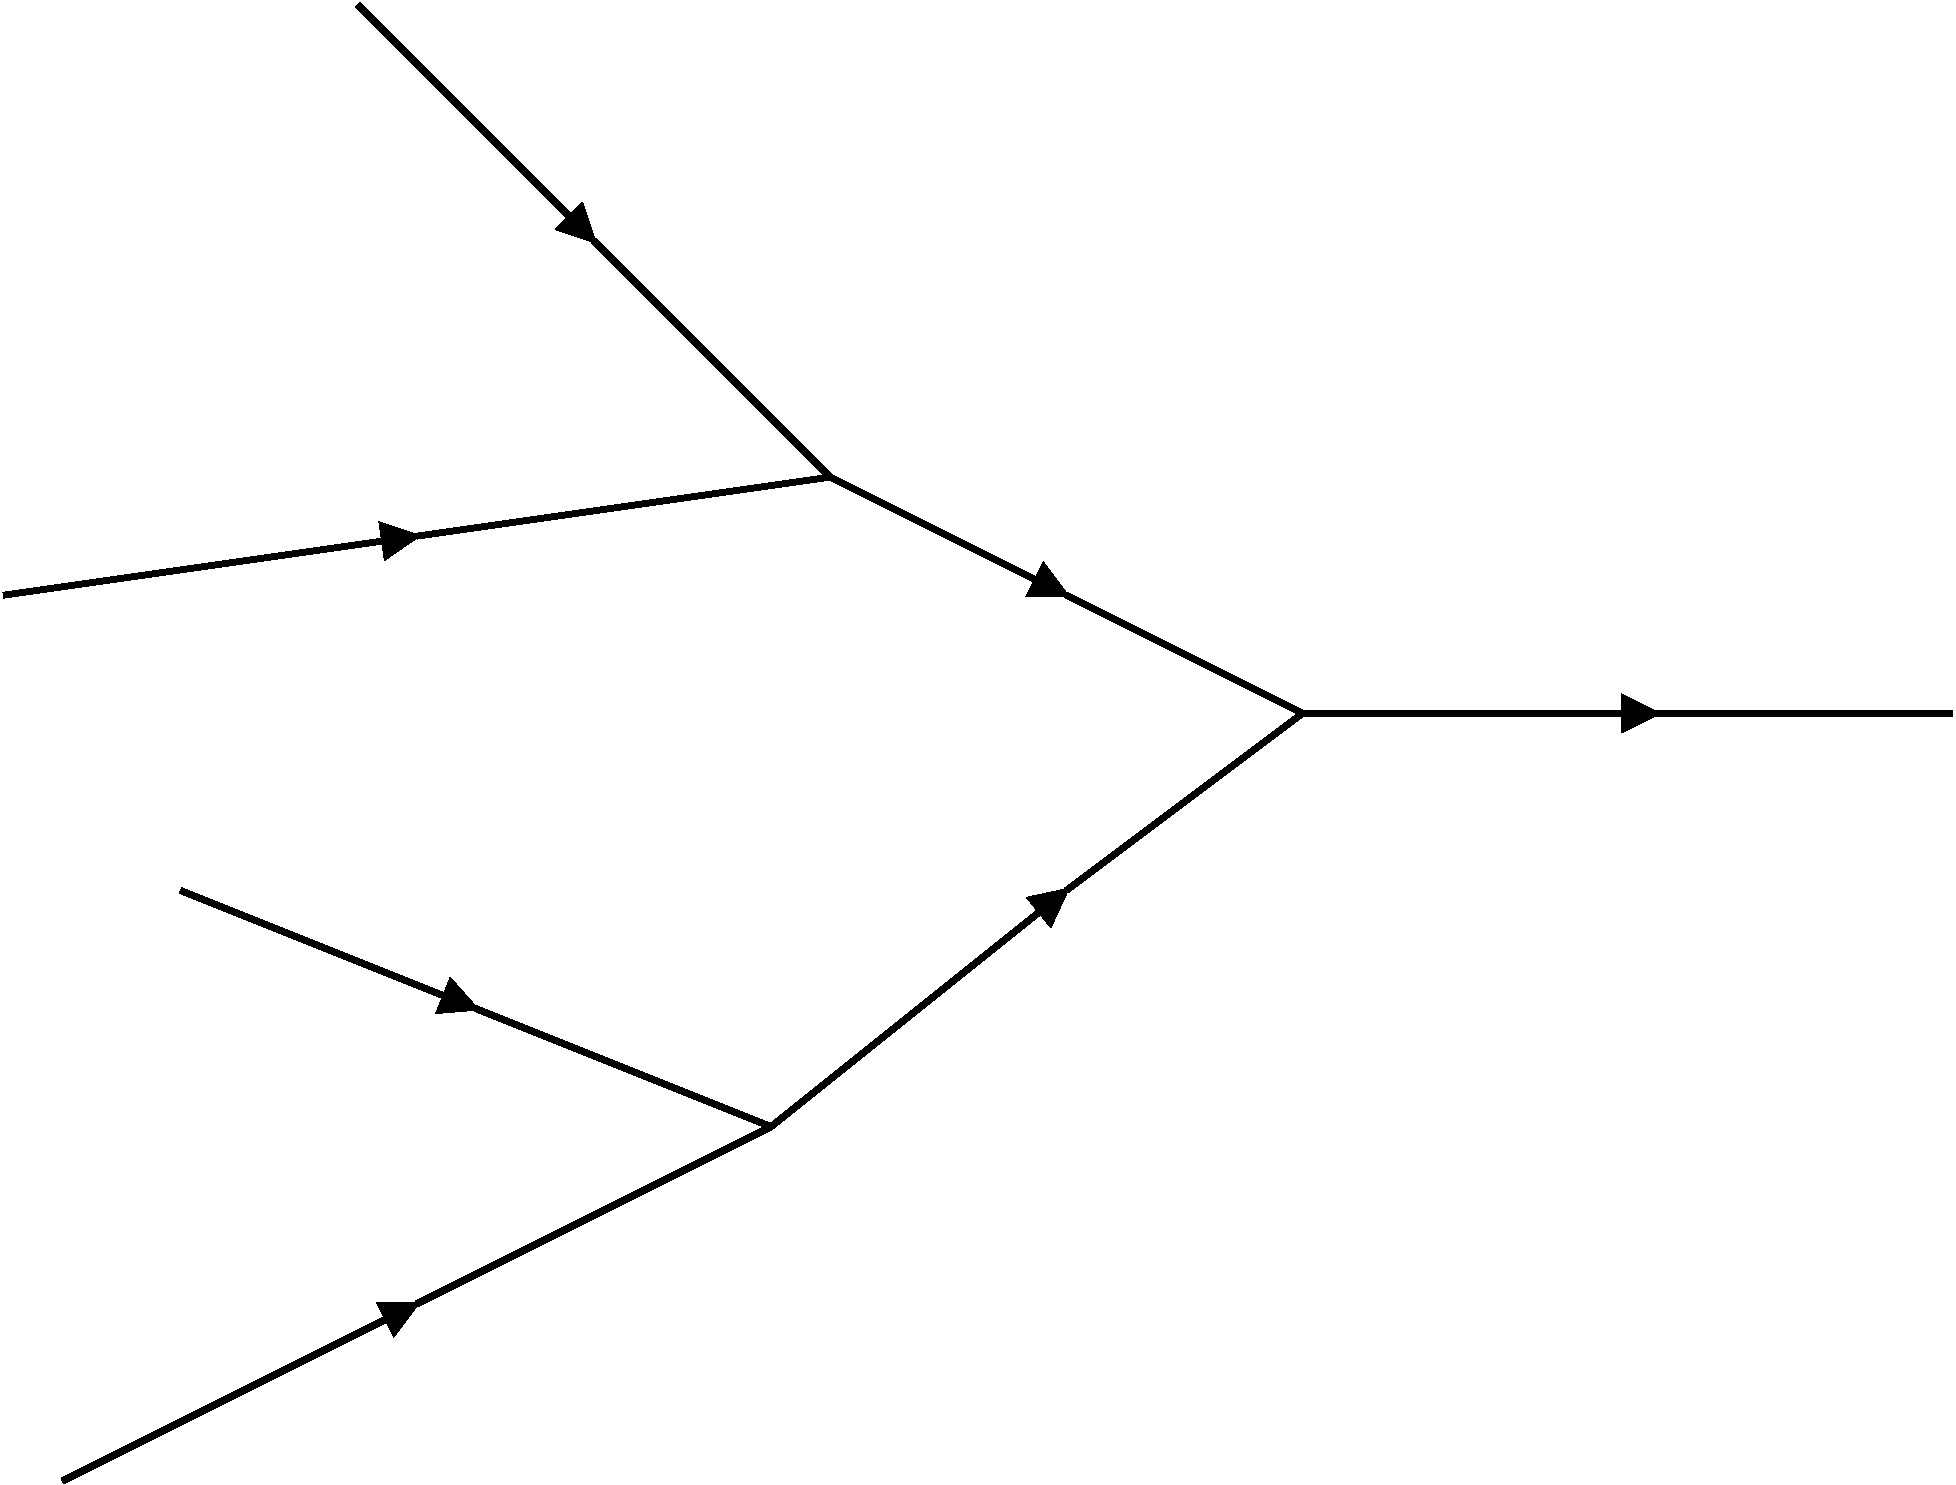
\includegraphics[width=0.6\columnwidth]{figures/stream_next_edge}
    \caption{Stream segmentation procedure network connectivity}
    \label{fig:stream_next_edge}
  \end{center}
\end{figure}

On the top of GRASS GIS provider a specialized GRASS {\em r.smoderp2d}
module has been designed. This tool allows a user running SMODERP2D
model computation directly from GRASS GIS working environment as
+demostrated in Figure~\ref{fig:r.smoderp2d}. The module can be easily
installed in GRASS GIS similarly to other extensions (so-called addons
modules) by {\em g.extension} command. By default, the {\em
  r.smoderp2d} module performs data preparation phase followed by
model computation steps. Data preparation only can be performed by
{\em -d} flag. In this case, the module creates a binary pickle file
which can be later used for a subsequent model computation. Note that
ArcGIS Toolbox also allows creating a pickle file for later
usage. Importantly, such pickle files are platform independent.

\begin{figure}[ht!]
  \begin{center}
    \includegraphics[width=1.0\columnwidth]{figures/smoderp2d_grass.png}
    \caption{Running r.smoderp2d module from GRASS GIS graphical user interface}
    \label{fig:r.smoderp2d}
  \end{center}
\end{figure}

{\em r.smoderp2d} command-line usage example:
\begin{verbatim}
r.smoderp2d elevation=w001001 soil=soil_map \
 soil_type=Novak vegetation=soil_map \
 vegetation_type=veg rainfall_file=rainfall.txt \
 points=points2 table_soil_vegetation=tab_sv \
 table_soil_vegetation_code=soilveg \
 table_stream_shape=tab_stream_shape \
 table_stream_shape_code=smoderp stream=stream 
\end{verbatim}

\subsubsection{QGIS plugin}
Recently the SMODERP2D model has been integrated also into QGIS
environment. QGIS\footnote{https://www.qgis.org} is a widely used open
source GIS platform which can be easily extended by user-defined
plugins. A SMODERP2D QGIS plugin allows performing both data
preparation and model computation phases in QGIS native environment,
see Figure~\ref{fig:smoderp2_qgis}. Data preprocessing is ensured by
GRASS GIS provider as described in \ref{sec:grass_provider}. Note that
QGIS installation normally comes with GRASS GIS included. It means
that GRASS dependency is solved by QGIS installation
itself. Experimental code of the plugin compatible with the current
long term release QGIS version 3.4 is available from the project GitHub
repository \cite{smoderp2d-github-2019}.

\begin{figure}[ht!]
  \begin{center}
    \includegraphics[width=1.0\columnwidth]{figures/smoderp2d_qgis.png}
    \caption{SMODERP2D model implemented as QGIS plugin}
    \label{fig:smoderp2_qgis}
  \end{center}
\end{figure}

\subsubsection{Python3 support}
SMODERP2D project also comes with Python 3 support, but still
supporting Python 2. Note that Python versions 2 and 3 are not
backwards compatible.  Python~3 support is important from various
perspectives. Python 2 is slowly reaching the end of
life\footnote{https://legacy.python.org/dev/peps/pep-0373/}, but is still used by many GIS platforms such as Esri ArcGIS 10.x. Newly supported
GIS platforms by the SMODERP2D project as Esri ArcGIS Pro, (upcoming)
GRASS GIS 7.8 and QGIS 3.x are Python 3 based. On the other hand it is
still meaningful to support both Python versions, Python 2 mainly
because of Esri ArcGIS 10.x platform.

\begin{figure}[ht!]
  \begin{center}
    \includegraphics[width=1.0\columnwidth]{figures/smoderp2d_arcgis.png}
    \caption{SMODERP2D model available as ArcToolbox for Esri ArcGIS
      10.x and Pro platforms}
    \label{fig:smoderp2d_arcgis}
  \end{center}
\end{figure}
